\documentclass[12pt]{article}  % [12pt] option for the benefit of aging markers

% amssymb package contains more mathematical symbols
\usepackage{amssymb,amsthm}
\usepackage{amsmath}
\usepackage{bm}

% graphicx package enables you to paste in graphics
\usepackage{graphicx}
\usepackage{auto-pst-pdf}
\usepackage{subfig}

% embed source inside latex
\usepackage[procnames]{listings}
\usepackage{color}

% page geometry
\usepackage{geometry}
\usepackage{array}

% ALGORITHM
\usepackage{algorithm}
\usepackage{algpseudocode}
\usepackage{hyperref}
\usepackage{booktabs}
\usepackage{enumitem}

%%%%%%%%%%%%%%%%%%%%%%%%%%%%%%%%%
%
%    Page size commands.  Don't worry about these
%
\setlength{\textheight}{220mm}
\setlength{\topmargin}{-10mm}
\setlength{\textwidth}{150mm}
\setlength{\oddsidemargin}{0mm}

%%%%%%%%%%%%%%%%%%%%%%%%%%%%%%%%%%%%%%%%%%%%%%%%%%%%%%%%%%%%%%%
%
%    Definitions of environments for theorems etc.
%
\newtheorem{theorem}{Theorem}[section]          % Theorems numbered within sections - eg Theorem 2.1 in Section 2.
\newtheorem{corollary}[theorem]{Corollary}      % Corollaries etc. will be counted as Theorems for numbering
\newtheorem{lemma}[theorem]{Lemma}              % eg Lemma 3.1, ... Theorem 3.2, ... Corollary 3.3.
\newtheorem{proposition}[theorem]{Proposition}
\newtheorem{conjecture}[theorem]{Conjecture}

\theoremstyle{definition}
\newtheorem{definition}[theorem]{Definition}

\theoremstyle{remark}
\newtheorem{remark}[theorem]{Remark}
\newtheorem{example}[theorem]{Example} 

%%%%%%%%%%%%%%%%%%%%%%%%%%%%%%%%%%%%%%%%%%%%%%%
%
%        Preamble material specific to your essay
%
\title{Modeling and Active Inferring Wireless Sensor Data}
\author{Yan Jiaqi A20321362\\
CS583 Project\\
supervised by
Mustafa Bilgic\\
Live Section
}

\begin{document}
\maketitle

% \newpage                     % optional page break
\begin{abstract}
Phase 1
\end{abstract}

% optional page break
\newpage
\tableofcontents

% optional page break
\newpage

\section{Phase 1}

\subsection{Model}
Every sensor's data at every timestamp is an isolated random variable.
Besides, they are represented as a Gaussian model:
\begin{align}
        p(X_{i,j}) = N(\mu_{i,j}, \sigma_{i,j}^2)
\end{align}
where $X_{i, j}$ is the random variable for sensor $i$'s data at time $j$.

\subsection{Phase 1 Experiment Results}
\label{sec:phase1:result}
See Figure~\ref{fig:phase1:temperature} and Figure~\ref{fig:phase1:humidity}.

\begin{figure}[H]
\centering
        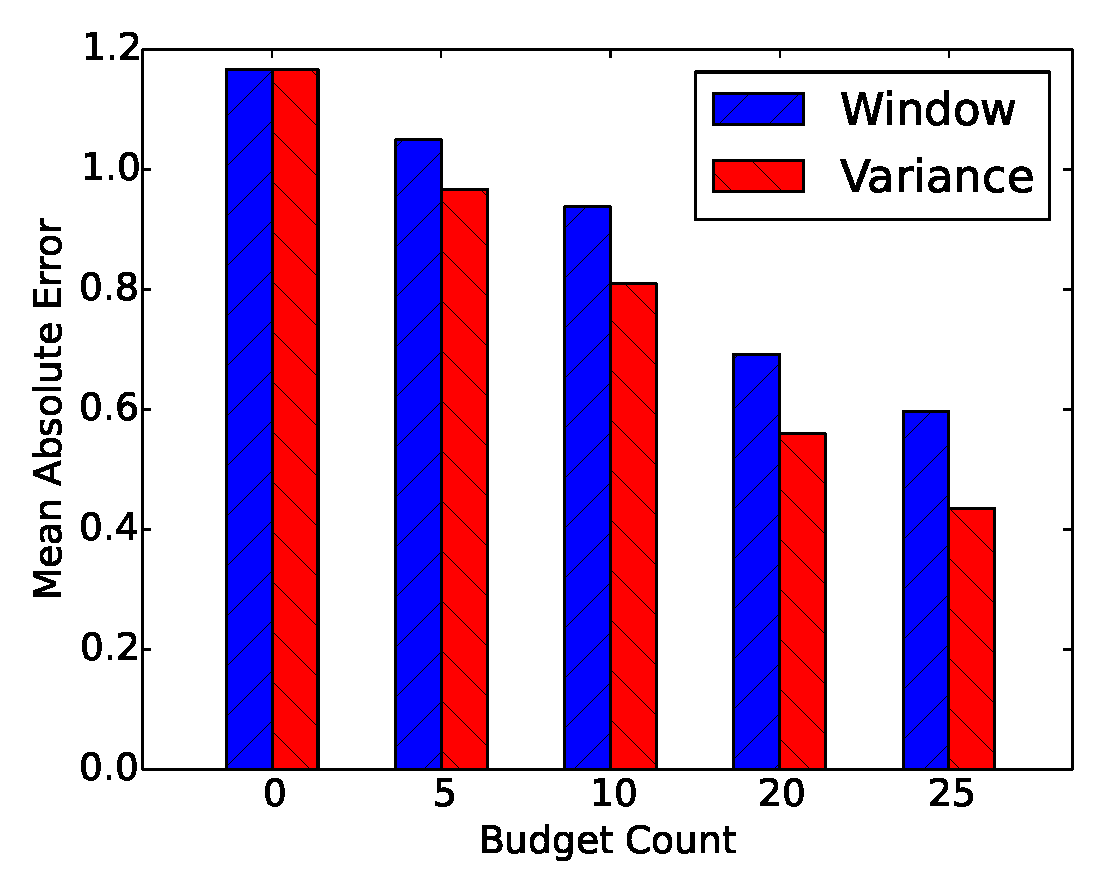
\includegraphics[width=0.58\textwidth]{../phase1/temperature_err}
        \caption{Inference Errors of \textbf{Temperature} Data at Different Budget Level}
\label{fig:phase1:temperature}
\end{figure}

\begin{figure}[H]
\centering
        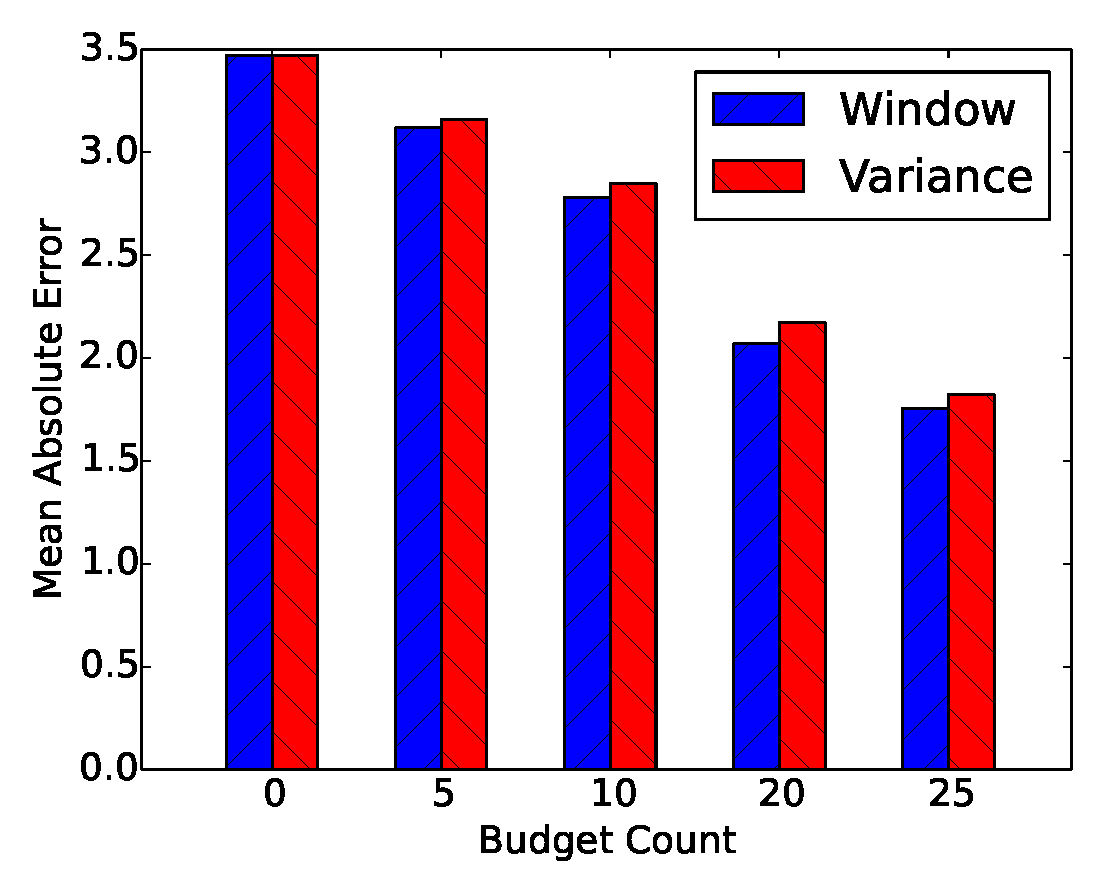
\includegraphics[width=0.58\textwidth]{../phase1/humidity_err}
        \caption{Inference Errors of \textbf{Humidity} Data at Different Budget Level}
\label{fig:phase1:humidity}
\end{figure}

\section{Phase 2}
For sensor $i$, the network model is a linear chain.
States are first-order Markovian.
\begin{align}
        & p(X_{i,j}|X_{i,j-1}) = N(\beta_0 + \beta_1 X_{i,j-1}, var_{X_{i,j}|X_{i,j-1}}) \\
        & p(X_{i,j}) = P(X_{i, j-1})P(X_{i,j}|X_{i, j-1})
\end{align}

\subsection{Hour Stationary Model}
If we assume hour stationary, the transition parameters are the same per sensor.
These parameters are learned by regression using all 3 day's data per sensor.
\begin{align}
        & \mu_{X_{i,j}} = \beta_{i,0} + \beta_{i,1} \mu_{X_{i,j}|X_{i,j-1}} \\
        & var_{X_{i,j}} = var_{X_{i,j}|X_{i,j-1}} + \beta_{i,1}^2 var_{X_{i,j-1}} 
\end{align}


\subsection{Day Stationary Model}
If we assume day stationary, the transition parameters are different inside one day,
but the same for timestamps across day.
For each transition parameters, 3 rows of data are used in regression.
\begin{align}
        & \mu_{X_{i,j}} = \beta_{i,j,0} + \beta_{i,j,1} \mu_{X_{i,j}|X_{i,j-1}} \\
        & var_{X_{i,j}} = var_{X_{i,j}|X_{i,j-1}} + \beta_{i,j,1}^2 var_{X_{i,j-1}} 
\end{align}
Transition parameters from one day to the next day are considered,
e.g.\ from hour 23.5 to 0.0 of the next day.
When learning these parameters, only 2 rows of train data are used in regression.
They are data from 1st day's 23.5 to 2nd day's 0.0,
and data from 2nd day's 23.5 to 3rd day's 0.0.


\subsection{Phase 2 Experiment Results}
\label{sec:phase2:result}
See Figure~\ref{fig:phase2:temperature} and Figure~\ref{fig:phase2:humidity}.

\begin{figure}[H]
\centering
        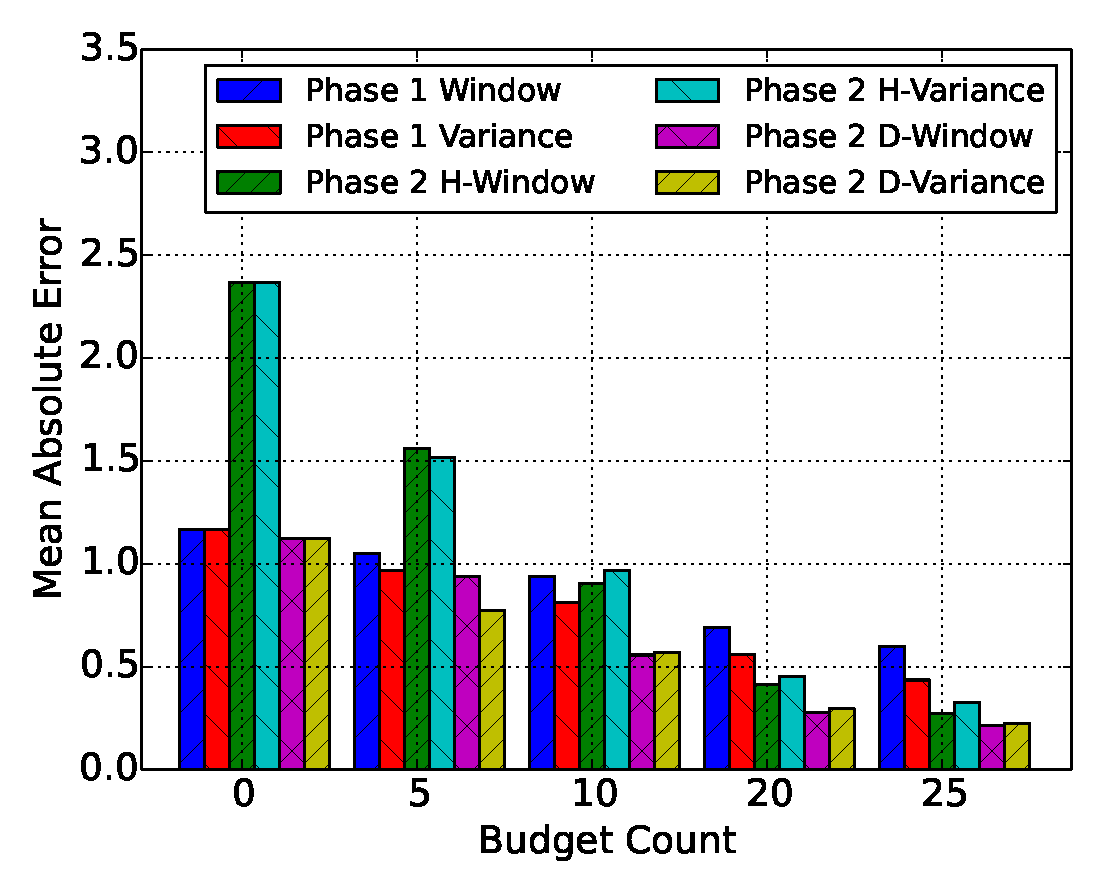
\includegraphics[width=0.58\textwidth]{../phase2/temperature_err}
        \caption{Inference Errors of \textbf{Temperature} Data at Different Budget Level}
\label{fig:phase2:temperature}
\end{figure}

\begin{figure}[H]
\centering
        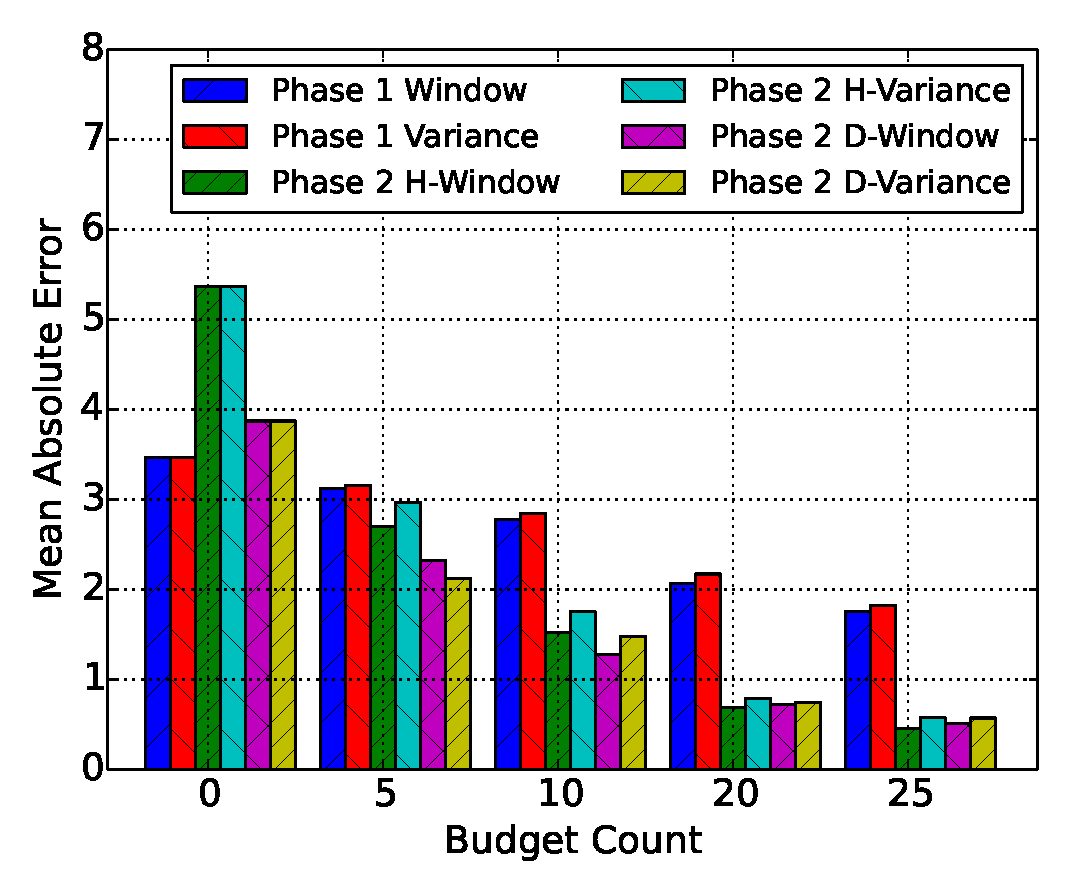
\includegraphics[width=0.58\textwidth]{../phase2/humidity_err}
        \caption{Inference Errors of \textbf{Humidity} Data at Different Budget Level}
\label{fig:phase2:humidity}
\end{figure}


\section{Phase 3 without Backward Inference}
\subsection{Model}
In phase 3, we assume hour-level stationary.
The model becomes more complicated since we consider the correlation between sensors:
\begin{align}
        p(X^{t}_i|\mathbf{X}^{t-1}) = \mathcal{N}(\beta_0 + \bm{\beta}\mathbf{X}^{t-1}; \sigma_i^2)
\end{align}
where $m=50$ is the number of sensors.
The prediction for sensor $i$ at time $j$ will be based on mean and variance:
\begin{align}
        & \mu_{X_{i,j}} = \beta_{i,0} + \sum_{k=1}^{m} \beta_{i,k} \mu_{X_{k,j-1}} \\
        & var_{X_{i,j}} = var_{X_{i,j}|X_{1,j-1},\ldots, X_{m,j-1}} + \sum_{k=1}^{m}\beta_{i,k}^2 var_{X_{k,j-1}}
\end{align}
$\bm{\beta}_i$ for sensor $i$ is learn by Lasso regression with $\alpha = 0.1$.
$\sigma_i^2$ is the regression variance.
Without considering observed data could influence backward,
the inference is the same as phase 2.

\subsection{Experiment Results}
See Figure~\ref{fig:phase3:temperature} and Figure~\ref{fig:phase3:humidity}.

\begin{figure}[H]
\centering
        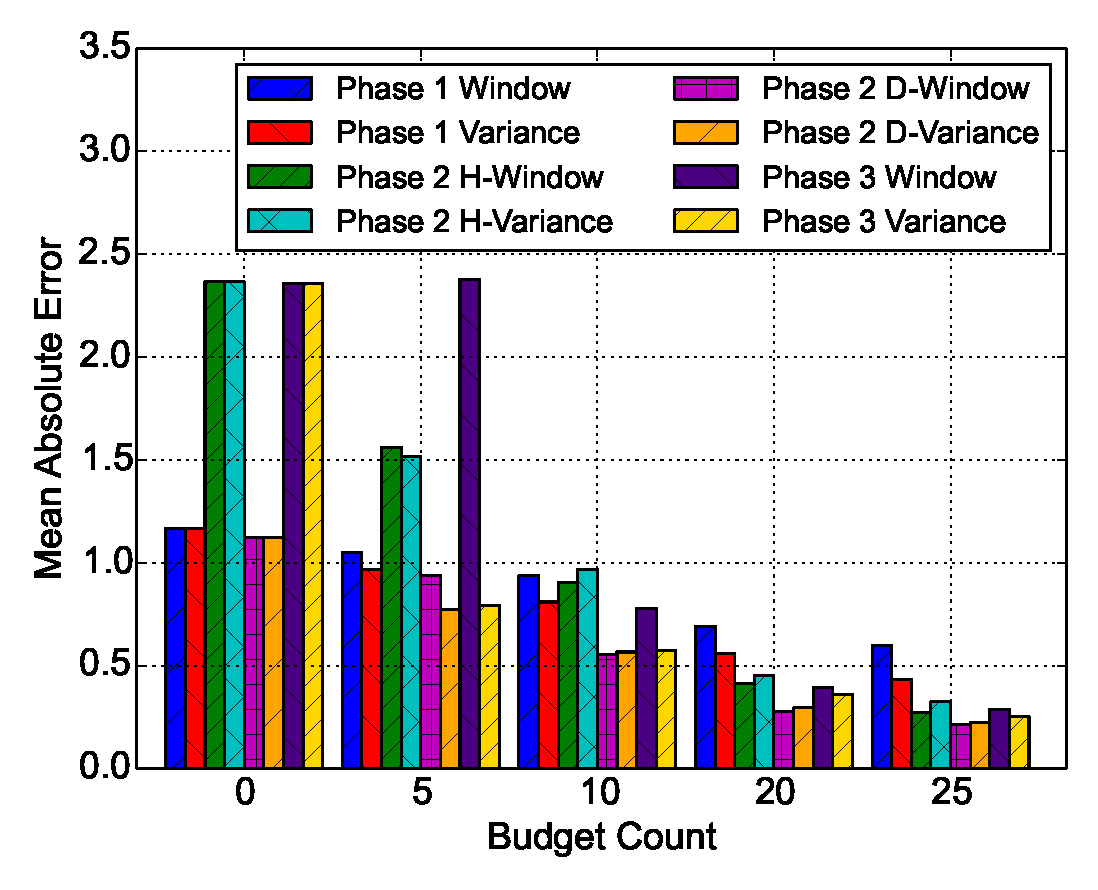
\includegraphics[width=0.58\textwidth]{../phase3/temperature_err}
        \caption{Inference Errors of \textbf{Temperature} Data at Different Budget Level}
\label{fig:phase3:temperature}
\end{figure}

\begin{figure}[H]
\centering
        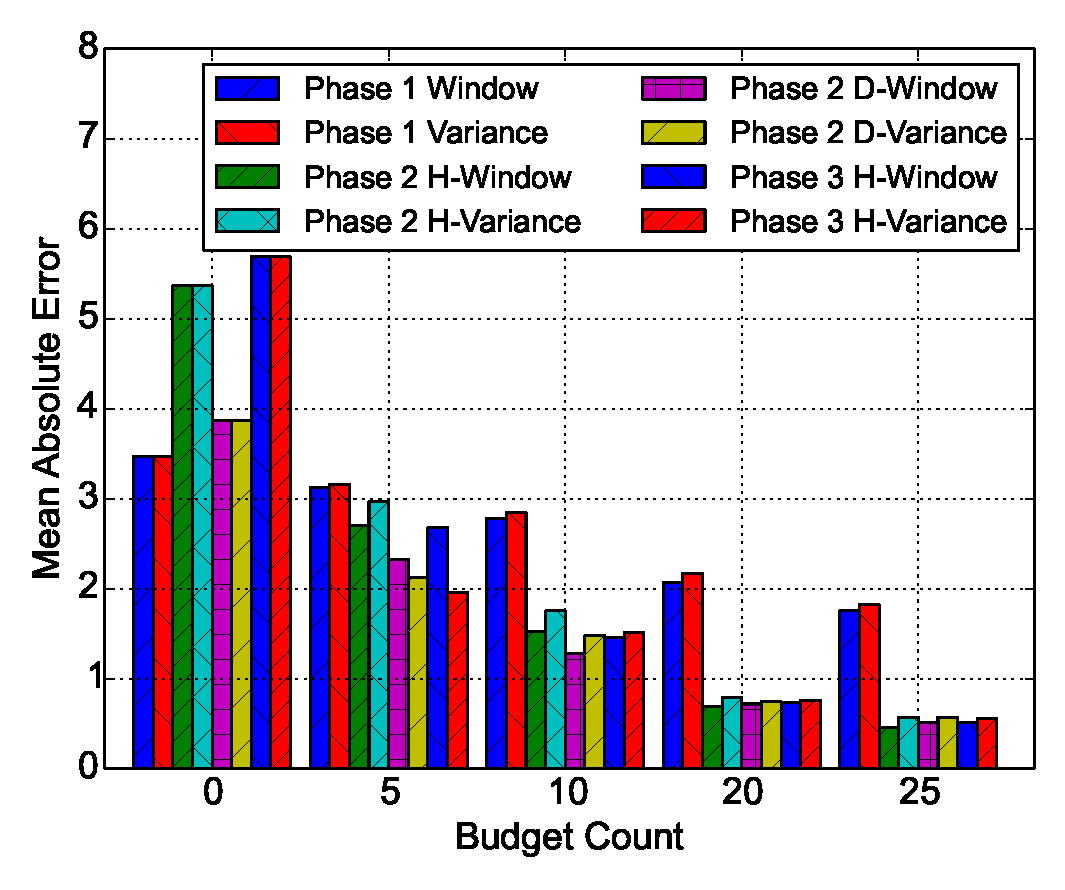
\includegraphics[width=0.58\textwidth]{../phase3/humidity_err}
        \caption{Inference Errors of \textbf{Humidity} Data at Different Budget Level}
\label{fig:phase3:humidity}
\end{figure}



\section{Phase 3 with Backward Inference}

\subsection{Model}
The Markovian temporal model for sensor $i$ is
\begin{align}
        P(\mathbf{X}^t | \mathbf{X}^{t-1}) = \mathcal{N}(A \mathbf{X}^{t-1}; Q) \\
\end{align}
where $\mathbf{X}$ is a $(m+1) \times 1$ vector, representing $m$ sensors and 1 imaginary parent
who's value is constant 1.
The parameters needed to be learned are
\begin{itemize}
        \item $A$: a $(m+1)\times (m+1)$ matrix describing the temporal transition relation
        \item $Q$: a $(m+1)\times (m+1)$ diagonal matrix describing the conditional variance
\end{itemize}
Lasso regression is used to learn these parameters.
Notice that in $A$ there is an parameter for intercept ($\beta_0$).
The first element in $Q$'s diagonal is zero, since the imaginary parent is always observed as 1.
For temperature data, $\alpha$ in Lasso regression is 0.09;
for humidity data, $\alpha$ in Lasso regression is 0.3.

\subsection{The Kalman Filter}
Inference using Kalman Filter contains two steps.
First, we have the normal \textit{state transition update}:
\begin{align}
        & \mu^{t} = A \mu^{t-1} \label{equ:transition:mu} \\
        & \Sigma^{t} = A\Sigma^{t-1}A^T + Q\label{equ:transition:sigma}
\end{align}
When we have a set of $k$ observed sensors $\mathbf{O}$ at $t+1$ time step,
we can update $\mu^{t}$ and $\Sigma^{t}$ using Kalman Gain:
\begin{align}
        & K^t = \Sigma^t H^T (H\Sigma^{t}H^T + R)^{-1} \\
        & \mu^t = \mu^t + K^t(\mathbf{O}^t - H\mu^t) \\
        & \Sigma^t = (I - K^t H)\Sigma^t 
\end{align}
where $H$ is $m+1$ by $k$ parameter matrix, extracted from the rows of observed sensor in $A$,
$R$ is $k$ by $k$ diagonal matrix constructed from $Q$ using the rows of the observed sensors,
$\mathbf{O}$ is a $k$ by 1 vector of observed sensor data.

Now we can use again Equation~\ref{equ:transition:mu} and Equation~\ref{equ:transition:sigma}
to predict the unobserved sensor at time $t+1$.
Notice that $k$ observations are used (e.g. $\mathbf{O}$ is a vector)
together to update last time step's means and variances.
If I do this backward update $k$ times iteratively, iteration will diverge.


\subsection{Experiment Results}
See Figure~\ref{fig:phase3_back_infer:temperature} and Figure~\ref{fig:phase3_back_infer:humidity}.

\begin{figure}[H]
\centering
        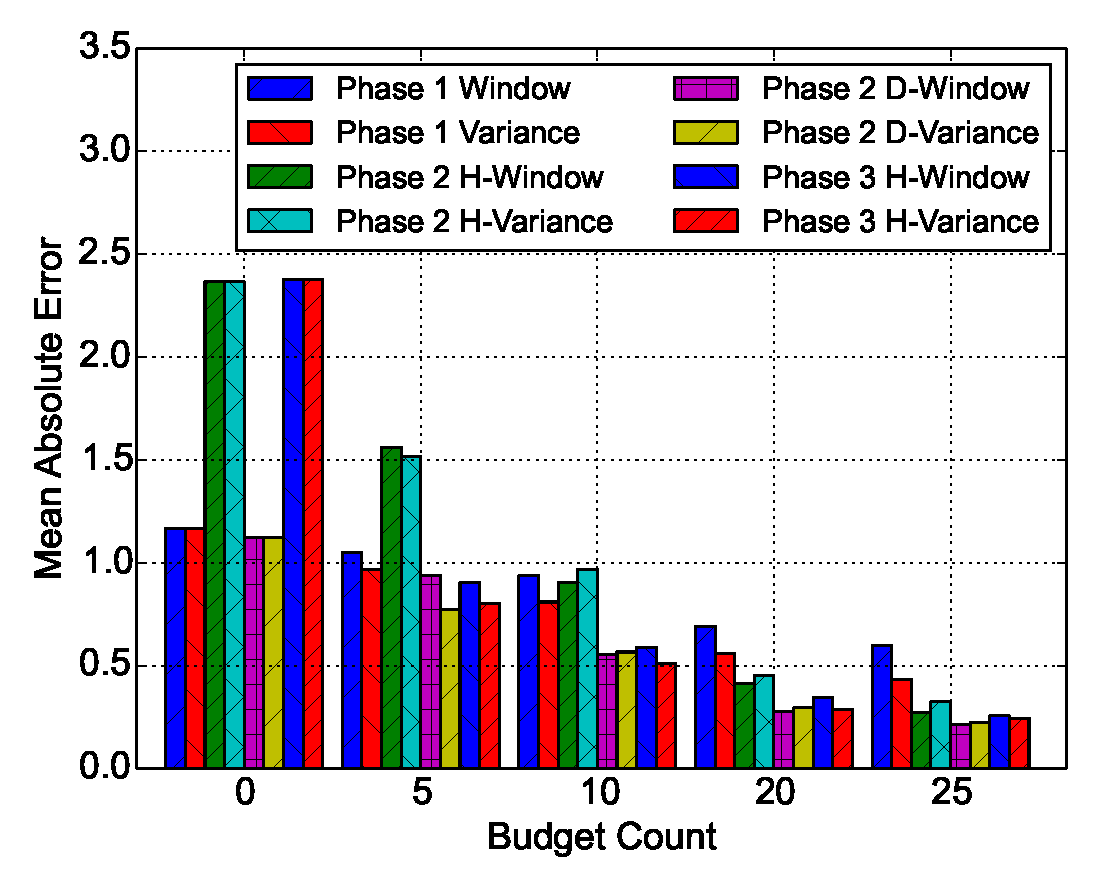
\includegraphics[width=0.58\textwidth]{../phase3_backinfer/temperature_back_infer_err}
        \caption{Inference Errors of \textbf{Temperature} Data at Different Budget Level}
\label{fig:phase3_back_infer:temperature}
\end{figure}

\begin{figure}[H]
\centering
        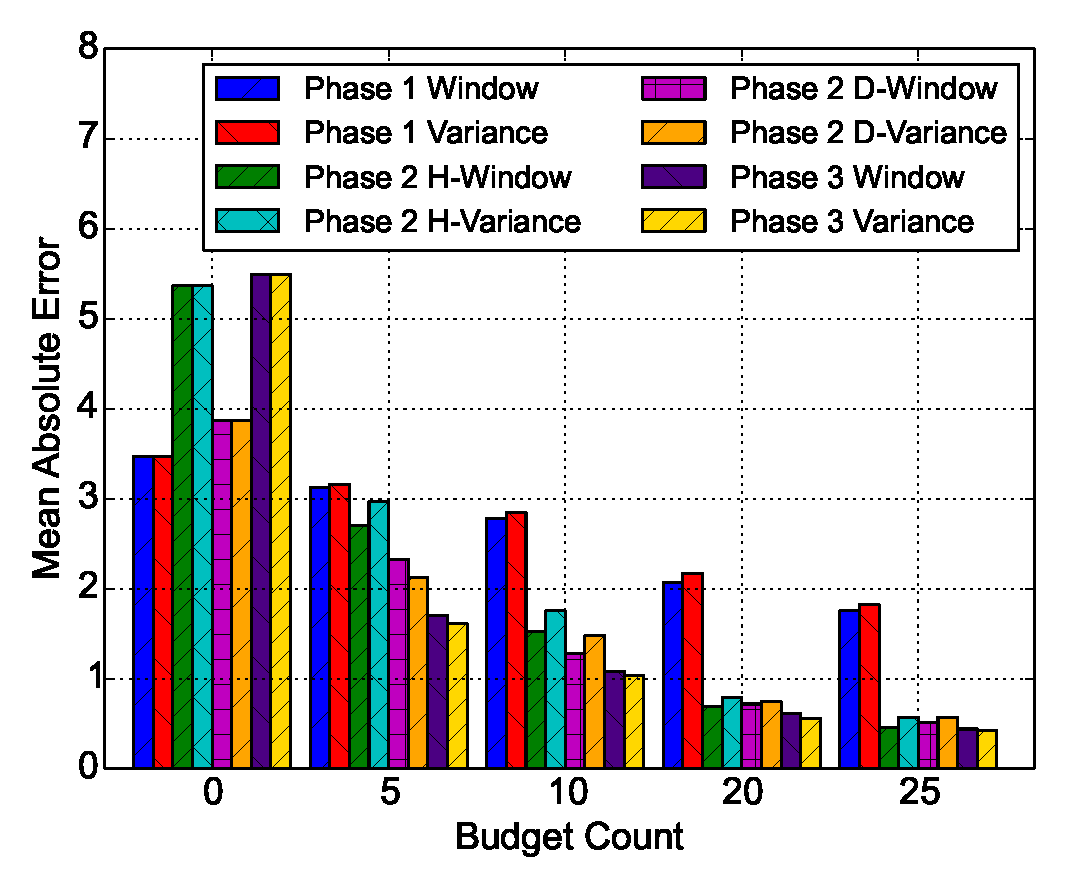
\includegraphics[width=0.58\textwidth]{../phase3_backinfer/humidity_back_infer_err}
        \caption{Inference Errors of \textbf{Humidity} Data at Different Budget Level}
\label{fig:phase3_back_infer:humidity}
\end{figure}


%%%%%%%%%%%%%%%%%%%%%%%%%%%%%%%%%%%%%%%%%
%
%     Bibliography
%
%     Use an easy-to-remember tag for each entry - eg \bibitem{How97} for an article/book by Howie in 1997
%     To cite this publication in your text, write \cite{How97}.  To include more details such as
%     page, Chapter, Theorem numbers, use the form \cite[Theorem 6.3, page 42]{How97}.
%
%\begin{thebibliography}{99}

% 
% The usual convention for mathematical bibliographies is to list alphabetically
% by first-named author (then second, third  etc. author then date)
% websites with no author names should go by the site name
%


% Typical layout for reference to a journal article
%
%\bibitem{Bovey}
%J. D. Bovey, M. M. Dodson,                         % author(s)
%The Hausdorff dimension of systems of linear forms % article name
%{\em Acta Arithmetica}                             % journal name - italics
%{\bf 45}                                           % volume number - bold
%(1986), 337--358.                                   % (year), page range

%% Typical layout for reference to a book
%%
%\bibitem{Cassels}
%J. W. S. Cassels,                                  % author(s)
%{\em An Introduction to Diophantine Approximation},% title - italics
%Cambridge University Press, Cambridge, 1965.       % Publisher, place, date.

%% Typical layout for reference to a website
%%
%\bibitem{GAP}
%The GAP Group, GAP -- Groups, Algorithms, and Programming,  % Site name
%Version 4.5.6; 2012. % other information
%(http://www.gap-system.org)  % URL


%% Typical layout for reference to an online article
%%
%\bibitem{Howie}
%J. Howie,                                            % author(s)
%{\em Generalised triangle groups of type $(3,5,2)$}, % article name - italics
%http://arxiv.org/abs/1102.2073                       % URL
%(2011).                                              % (year)
%\end{thebibliography}

\end{document}
